%\documentclass{article}
%\usepackage{graphicx} % Required for inserting images
%\graphicspath{{figs/}}
%\usepackage{gensymb}
%\usepackage{tfrupee}
%\usepackage{amsmath}
%\title{GEOMETRY}
%\begin{document}
%\maketitle
%\begin{enumerate}
    \item What is the length of the arc of the sector of a circle with radius $14$ cm and of central angle $90\degree$.
    \begin{enumerate}
        \item $22$ cm
        \item $44$ cm
        \item $88$ cm
        \item $11$ cm
    \end{enumerate}
    \item if$\triangle ABC \sim \triangle PQR$ with $\angle A=32\degree$ and $\angle R=65\degree$,then the measure of $\angle B$ is:
    \begin{enumerate}
        \item $32\degree$
        \item $65\degree$
        \item $83\degree$
        \item $97\degree$
    \end{enumerate}
    \item What is the total surface area of a solid hemisphere of diameter $'d'$?
    \begin{enumerate}
        \item $3 \pi d^2$
        \item $2 \pi d^2$
        \item $\frac{1}{2} \pi d^2$
        \item $\frac{3}{4} \pi d^2$
    \end{enumerate}
    \item In $\triangle ABC$,$DE \parallel BC$.if $AD=2$ units,$DB=AE=3$ units and $EC=x$ units,then the value of $x$ is :
    \begin{figure}[!ht]
        \centering
        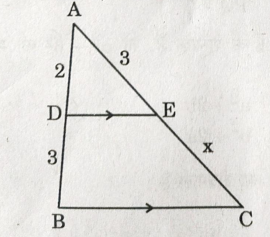
\includegraphics[width=\columnwidth]{figs/30-2-1-question12.png}
        \caption{$\triangle ABC$}
        \label{fig:enter-label1}
    \end{figure}
            \begin{enumerate}
                \item $2$
                \item $3$
                \item $5$
                \item $\frac{9}{2}$
            \end{enumerate}
    \item A straight highway leads to the foot of a tower.A man standing on the top of the $75$ m high tower observes two cars at angles of depression of $30\degree$ and $60\degree$,Which are approaching the foot of the tower.If one car is exactly behind the other on the same side of the tower,find the distance between the two cars.
    \item From the top of a $7$ m high building, the angle of elevation of the top of a cable tower is $60\degree$ and the angle of depression of its foot is $30\degree$.Determine the height of the tower.(take $\sqrt{3}=1.73$)
    \item Governing council of local public development authority of Dehradun decided to build and adventurous playground on the top of a hill,Which will have adequate space for parking.
    After survey,it was decided to build rectangular playground,with a semi-circular area allocated for parking at one end of the playground.The length and breadth of the rectangular playground are $14$ units and $7$ units,respectively.There are two quadrants of radius $2$ units on one side for special seats:
            \begin{enumerate}
                \item What is the total perimeter of the parking area?
                \item What is the total area of parking and the two quadrants?
                \item What is the ratio of area of playground to the area of parking area?
                \item Find the cost of fencing the playground and parking area at the rate of \rupee $2$ per unit.
            \end{enumerate}
    \begin{figure}[!ht]
        \centering
        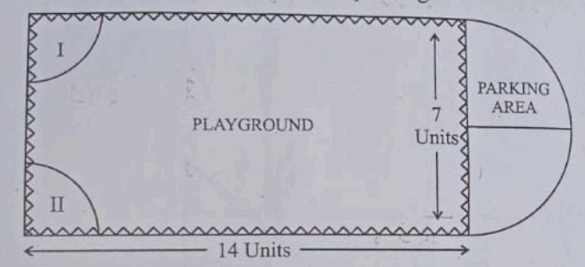
\includegraphics[width=\columnwidth]{figs/30-4-3-question36.png}
        \caption{Playground}
        \label{fig:enter-label2}
    \end{figure}
\end{enumerate}
%\end{document}
